%% LyX 2.4.0~RC3 created this file.  For more info, see https://www.lyx.org/.
%% Do not edit unless you really know what you are doing.
\documentclass[twocolumn,spanish,aps,prl,groupedaddress]{revtex4-2}
\usepackage[T1]{fontenc}
\usepackage[utf8]{inputenc}
\setcounter{secnumdepth}{3}
\usepackage{amsmath}

\makeatletter
%%%%%%%%%%%%%%%%%%%%%%%%%%%%%% User specified LaTeX commands.
\usepackage{graphicx}
\usepackage{epstopdf}
%\usepackage{amsmath}% http://ctan.org/pkg/amsmath
%\usepackage{amsthm}
%\usepackage{amsfonts}
%\usepackage{subfigure}
%\usepackage{hhline}
%\usepackage[miktex]{gnuplottex}
%\usepackage{xcolor}
\usepackage{amssymb}
\usepackage{amsmath}
\usepackage{color}
\usepackage{hyperref}
%\usepackage[percent]{overpic}
\usepackage{tikz}
\usepackage{mathrsfs}
\usepackage{wasysym}
\usepackage{tikz-cd}
%\usepackage{stix} %\fisheye
\usepackage{stackengine,scalerel}

% so sections, subsections, etc. become numerated.
\setcounter{secnumdepth}{3}

\newcommand{\avrg}[1]{\left\langle #1 \right\rangle}
\newcommand{\nelta}{\bar{\delta}}
\newcommand{\bra}[1]{\left\langle #1\right|}
\newcommand{\ket}[1]{\left| #1 \right\rangle}
\newcommand{\sbra}[1]{\langle #1|}
\newcommand{\sket}[1]{| #1 \rangle}
\newcommand{\bek}[3]{\left\langle #1 \right| #2 \left| #3 \right\rangle}
\newcommand{\sbek}[3]{\langle #1 | #2 | #3 \rangle}
\newcommand{\braket}[2]{\left\langle #1 \middle| #2 \right\rangle}
\newcommand{\ketbra}[2]{\left| #1 \middle\rangle \middle\langle #2  \right|}
\newcommand{\sbraket}[2]{\langle #1 | #2 \rangle}
\newcommand{\sketbra}[2]{| #1 \rangle  \langle #2 |}
\newcommand{\norm}[1]{\left\lVert#1\right\rVert}
\newcommand{\snorm}[1]{\lVert#1\rVert}
\newcommand{\bvec}[1]{\boldsymbol{\mathsf{#1}}}
\newcommand{\bcov}[1]{\boldsymbol{#1}}
\newcommand{\bdua}[1]{\boldsymbol{\check{#1}}}
%\newcommand{\bdov}[1]{\boldsymbol{\breve{#1}}}
\newcommand{\bdov}[1]{\breve{#1}}
%\newcommand{\bten}[1]{\boldsymbol{\mathfrak{#1}}}
\newcommand{\bten}[1]{\boldsymbol{\mathfrak{#1}}}
\newcommand{\forany}{\tilde{\forall}}
\newcommand{\qed}{$\overset{\circ}{.}\;$}

\newcommand\bigeye{\ensurestackMath{\stackinset{c}{}{c}{-.3pt}%
  {\bullet}{\scriptstyle\bigcirc}}}
\newcommand\eye{\scalerel*{\bigeye}{x}}
%\newcommand*{\fisheye}{%
%    \mathbin{%
%        \ooalign{$\circledcirc$\cr\hidewidth$\bullet$\hidewidth}%
%    }%
%}
\renewcommand{\appendixname}{Apéndice} % Change "Appendix" to "Apéndice"
\renewcommand{\fnum@figure}{Fig.~\thefigure} 

\makeatother

\usepackage{babel}
\addto\shorthandsspanish{\spanishdeactivate{~<>.}}
\deactivatequoting

\begin{document}
\title{Modelo Hodgkin \& Huxley}
\author{Adolfo Banchio}
\email{adolfo.banchio@mi.unc.edu.ar}

\author{Alejandro Matias Toledo}
\email{amtoledo2002@mi.unc.edu.ar}

\affiliation{Facultad de Matemática, Astronomía, Física y Computación, Universidad
Nacional de Córdoba}
\date{\today}
\begin{abstract}
En este trabajo se estudia el comportamiento de una neurona desde
un enfoque teórico, utilizando el modelo matemático de Hodgkin y Huxley.
Este modelo describe la propagación del potencial de acción a partir
del funcionamiento de los canales iónicos en la membrana neuronal.
Se realizaron simulaciones numéricas del modelo para analizar propiedades
clave del potencial de acción. Este trabajo es importante para comprender
los mecanismos fundamentales de la excitación neuronal y su propagación.
\end{abstract}
\maketitle

\section{INTRODUCCIÓN}

Las neuronas son las células encargadas de transmitir la información
en organismos complejos a través de señales eléctricas, estos mensajes
se conocen como el potencial de acción. Nace en la propia neurona
y se va propagando de una a otra hasta alcanzar el destino objetivo,
este sera nuestro objeto de estudio para este trabajo. Lo estudiaremos
a partir del modelo propuesto por Hodgking y Huxley en el año 1952
realizando simulaciones numéricas del sistema, con el objetivo de
estudiar la célula desde un punto de vista de un sistema dinámico.
Buscaremos contestar preguntas como <<¿Que hace disparar una neurona?>>.~\cite{HodgkinHuxleyModel}~\cite{izhikevich2006}

\section{TEORÍA}

El modelo de H\&H propuesto trata de explicar el funcionamiento de
la neurona como capacitores donde la diferencia de potencial eléctrico
entre el exterior y el interior se da debido a diferentes concentraciones
de cargas iónicas. Considerando que las neuronas poseen dos canales,
uno de sodio con dos compuertas (entrada y salida) y otro de potasio
con una única compuerta. El sistema puede ser descrito por las siguientes
ecuaciones diferenciales. {\small\begin{eqnarray*}
\dot{n}&=&\alpha_n(v)(1-n)-\beta_n(v) n\\
\dot{m}&=&\alpha_m(v)(1-m)-\beta_m(v) m\\
\dot{h}&=&\alpha_h(v)(1-h)-\beta_h(v) h \\
\dot{v}&=&c^{-1}(i-\bar{g}_{\mathrm{Na}}m^3h(v-v_{\mathrm{Na}})-\bar{g}_{\mathrm{K}}n^4(v-v_{\mathrm{K}})-g_{l}(v-v_{l}))
\end{eqnarray*}}{\small\par}

Donde n representa la fracción de compuertas de potasio abiertas,
m la fracción de compuertas de activación de sodio abiertas y h la
fracción de compuertas de inactivación abiertas. Para cada caso $\alpha_{k}$
y $\beta_{k}$ representan la tasa de apertura y clausura de cada
tipo de compuerta respectivamente;v representa el potencial eléctrico
de la membrana neuronal e i la corriente externa que estimula a la
neurona. Las ecuaciones y valores de los parámetros están desarrollados
en ~\cite{izhikevich2006}.

En este trabajo integraremos numéricamente dichas ecuaciones en pos
de poder representar el comportamiento del sistema bajo el estimulo
de diferentes corrientes externas. 

\section{RESULTADOS}

El primero de los análisis realizados fue el de encontrar los valores de
equilibrio de las cuatro variables involucradas en nuestro sistema (v, m, n, h).
Para ello integramos numéricamente partiendo desde una condición inicial
de 0 para cada variable. ver fig.~\ref{fig:fig1}. 

\begin{figure}[hb]
    \centering
    \includegraphics[width=0.85\linewidth]{Informe/graficos/ejercicio_3.png}
    \caption{Caption}
    \label{fig:fig1}
\end{figure}

En general los siguientes escenarios simulados partirán desde la condición inicial de los valores de equilibrio y variaran la función que representa la corriente externa del sistema.

\subsection{Estimulo débil y estimulo fuerte}

Los estímulos aplicados a la neurona para este experimento fueron de (\(10\mu A /cm^2\)) y (\(30\mu A /cm^2\)) con una duración de \(0.5ms\) espaciados por (\(8ms\)).

En la figura ~\ref{fig:fig2} podemos notar que en el primer impulso, en t=2ms, se produce un estimulo débil que no es suficiente para que la neurona se active. En cambio,
en el segundo impulso, el estimulo es suficiente para que la neurona dispare. 
Observando el comportamiento de las compuertas en el primer impulso, la fracción de compuertas de sodio activadas (m) aumenta y la fracción de compuertas de inactivación (h) disminuye, en cambio, la fracción de compuertas de potasio activados (n) aumenta lentamente. Todas las compuertas intentan volver a su estado de equilibrio.

En el siguiente impulso ocurre un disparo, por lo que la fracción de compuertas n,m y h  se comporta de manera esperada durante la ocurrencia de un potencial de acción. Y luego vuelven a sus valores de equilibrio.

\begin{figure}[h!]
    \centering
    \includegraphics[width=0.90\linewidth]{Informe/graficos/ejercicio_4.png}
    \caption{Caption}
    \label{fig:fig2}
\end{figure}

\subsection{Ráfaga}

Aplicamos un estimulo constante (\(10\mu A /cm^2\)) transcurridos 5ms. En la figura ~\ref{fig:fig3} observamos que la neurona responde generando una serie de potenciales de acción repetidos a partir del primer tiempo de estimulo (\(5ms\)). 

Al tener un estimulo constante vemos que las compuertas responden de manera mas lenta a diferencia de cuando luego de un potencial de acción no existen mas estímulos (ver fig~\ref{fig:fig2}). Hasta que finaliza el periodo refractario y la neurona vuelve a disparar.

\subsection{Período Refractario}
En este escenario, se aplicó un estímulo intermitente, con una duración de 2
ms cada 10 ms, dada por la siguiente función para la corriente externa.

$\small
i(t)=\begin{cases}
10\mu A/cm^{2} & t\in[10ms,10ms\:k+2],k\in\{1,2,3,4,..\}\\
0 & c.c.
\end{cases}$
\par 

La neurona disparó durante el primer estímulo, pero en el siguiente estimulo no fue capaz de generar otro potencial de acción. Esto puede verse reflejado en la figura ~\ref{fig:fig4}.
Ahora bien, esto sucede ya que luego de cada disparo la neurona mantiene las compuertas iónicas, 
especialmente las de sodio, inactivas, imposibilitando un nuevo disparo, 
a esto es lo que denominamos un periodo refractario. 
A medida que se recuperan las compuertas activas, el estímulo puede generar un nuevo potencial de acción si es suficientemente fuerte.
En este caso de estudio, un estimulo cada 10ms no es suficiente para que el periodo refractario cese, por lo que surge este comportamiento observado, de que un estimo provoca un potencial de acción y el siguiente no (ya que se encuentra dentro en el periodo refractario del anterior estimulo).

\subsection{Excitaciones con ruido}

En este caso la corriente es estocástica tal que $i(t)\sim i_{0}N(0,1)$
donde establecemos $i_{0}=50$. Y los resultados obtenidos para este
caso se ven en fig ~\ref{fig:fig5}. 

Este tipo de comportamiento intenta reflejar una situación mas realista, ya que las neuronas no reciben estímulos constantes ni en ráfaga, sino que responden a estímulos que varían según el entorno planteado. 
Podemos observar que la neurona responde de la misma manera a los casos planteados anteriormente.
Solamente genera un potencial de acción cuando el estimo corresponde a una corriente lo suficientemente potente para que la neurona dispare.

\section{DISCUSIÓN}

\section{CONCLUSIONES}

A pesar de la variabilidad, el modelo neuronal sigue siendo capaz de responder de manera coherente, 
mostrando el robusto diseño del sistema Hodgkin-Huxley.

\section{AGRADECIMIENTOS}

\bibliographystyle{apsrev4-2}
\bibliography{ref}

\begin{figure}[b]
  \centering
  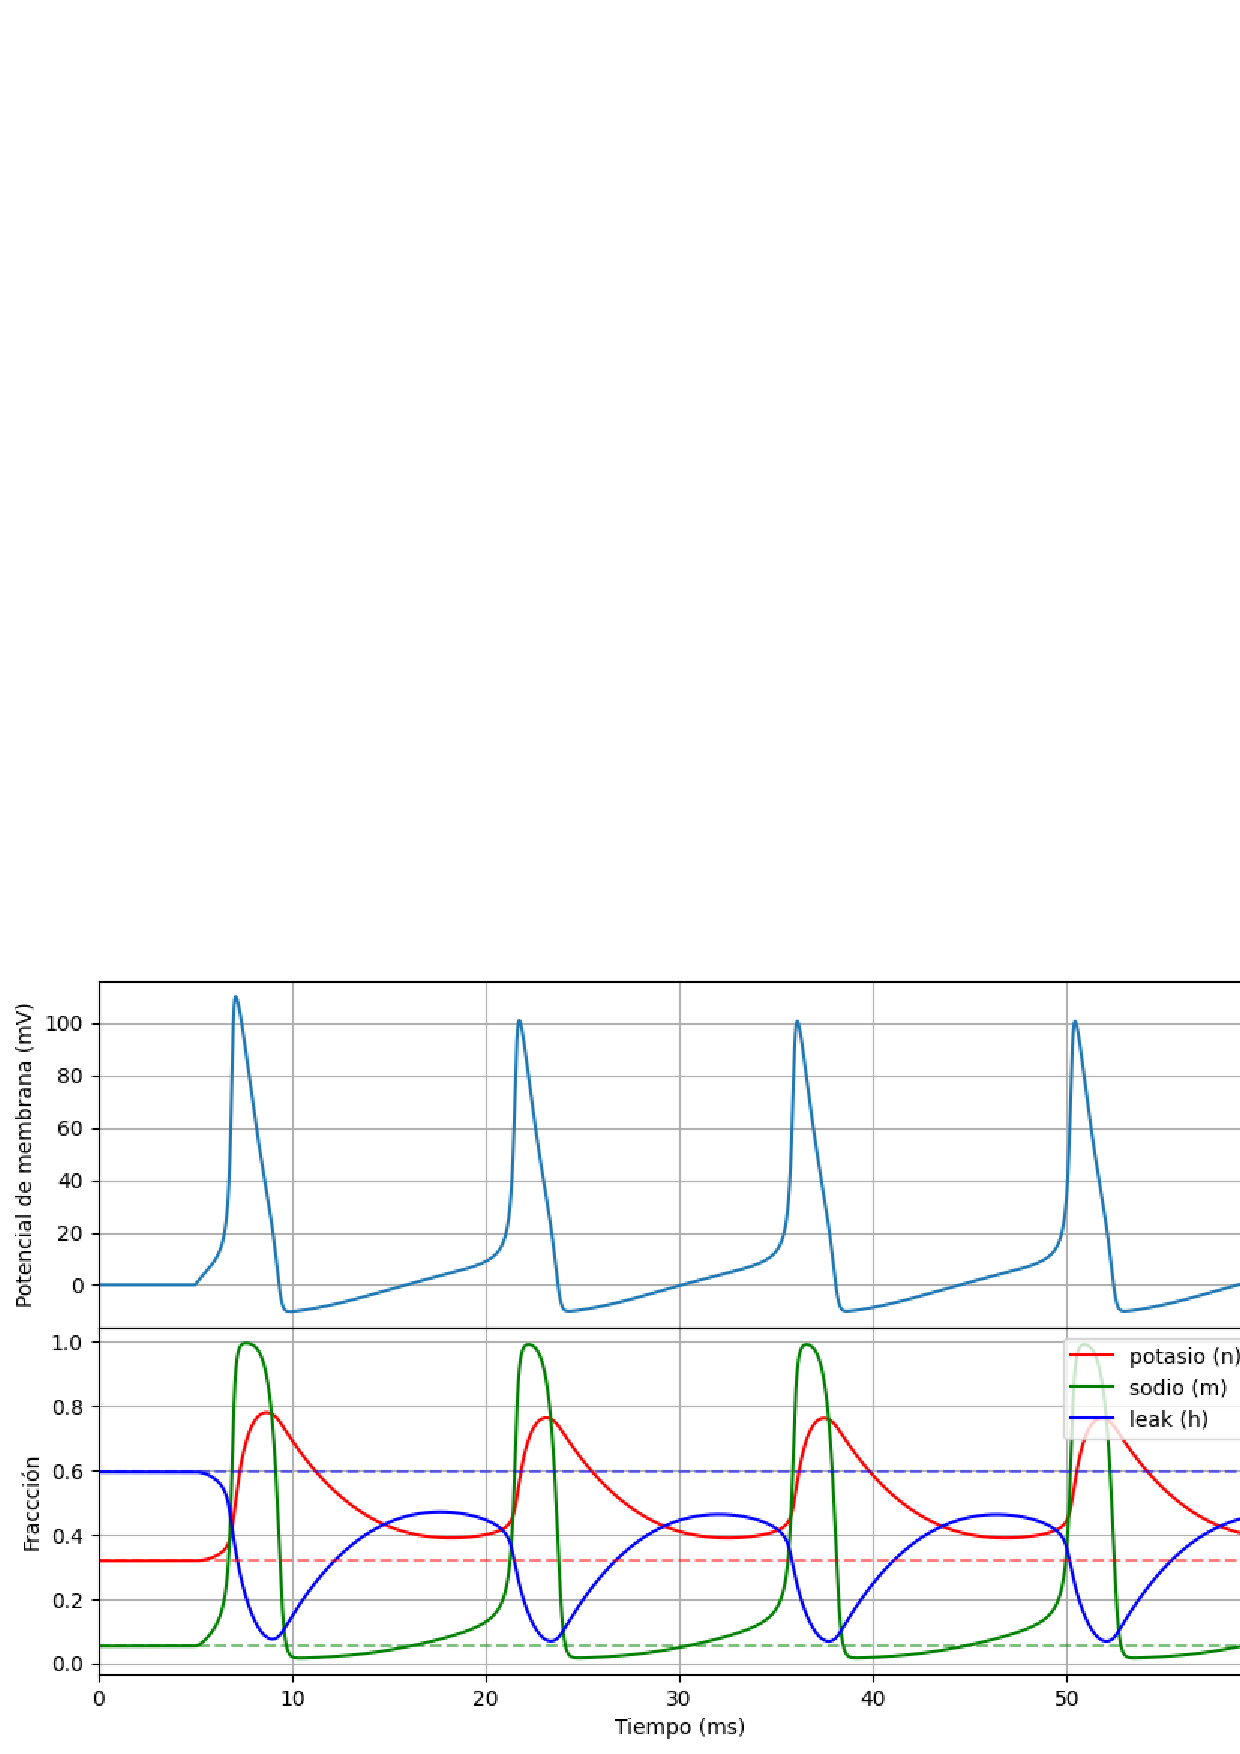
\includegraphics[width=0.90\textwidth]{graficos/ejercicio_5.png}
  \caption{Gráfico correspondiente al caso de ráfaga. Frente a un estimulo se representan el valor de el potencial de la membrana y los valores de las fracciones de las compuertas.}
  \label{fig:fig3}

  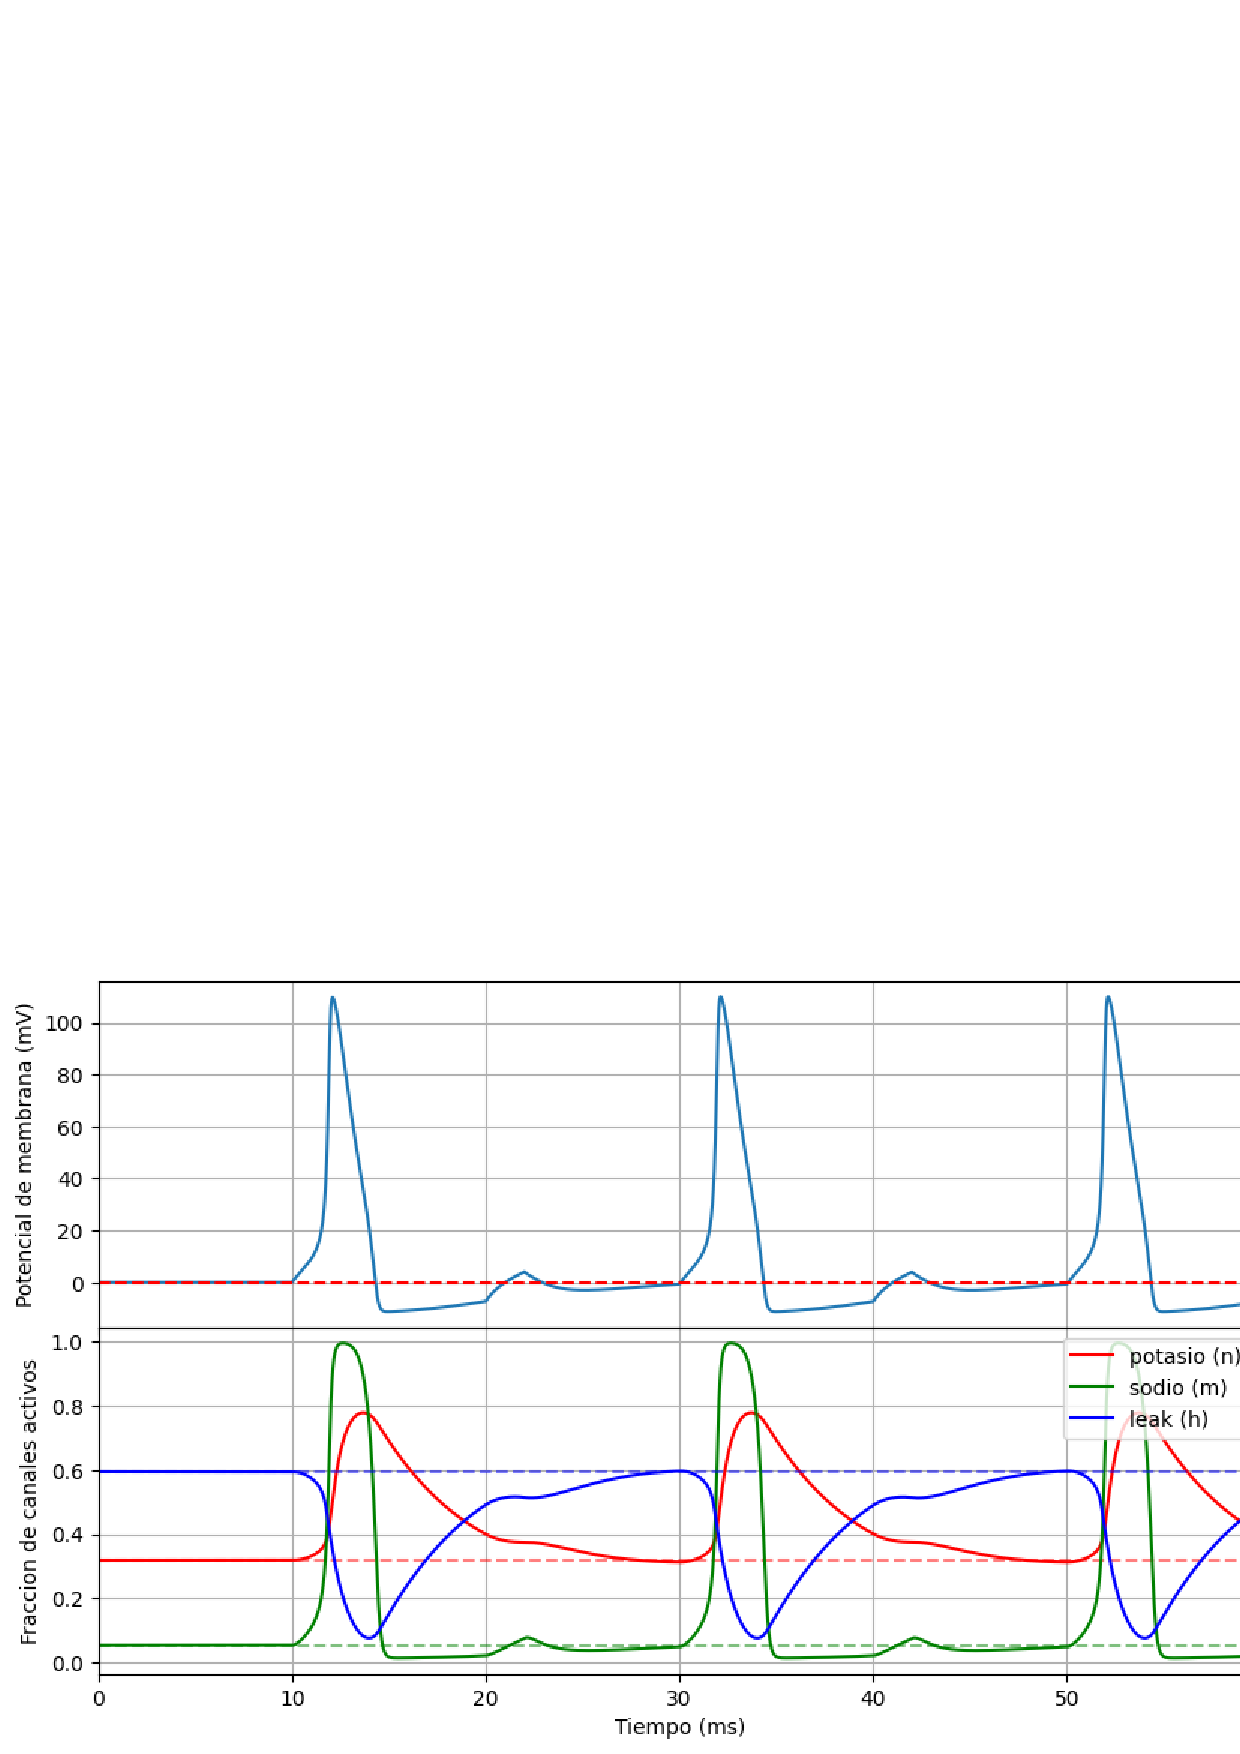
\includegraphics[width=0.90\textwidth]{graficos/ejercicio_6.png}
  \caption{Gráfico correspondiente al caso de periodo refractario. Frente a un estimulo se representan el valor de el potencial de la membrana y los valores de las fracciones de las compuertas.}
  \label{fig:fig4}
\end{figure}

\begin{figure}
    \centering
    \includegraphics[width=0.9\textwidth]{Informe/graficos/ejercicio_7.png}
    \caption{Gráfico correspondiente al caso de excitaciones con ruido. Frente a un estimulo se representan el valor de el potencial de la membrana y los valores de las fracciones de las compuertas.}
    \label{fig:fig5}
\end{figure}

\end{document}